\documentclass[12pt, oneside]{article} 
\usepackage{amsmath, amsthm, amssymb, calrsfs, wasysym, verbatim, bbm, color, graphics, geometry}
\usepackage{mathtools}
\usepackage{hyperref}

\geometry{tmargin=.75in, bmargin=.75in, lmargin=.75in, rmargin = .75in}  
\setlength{\parindent}{0in}
\setlength{\parskip}{\baselineskip}%
\setlength{\parindent}{1.5pt}%
\DeclareMathOperator*{\argmax}{argmax} % thin space, limits underneath in displays

\newcommand{\R}{\mathbb{R}}
\newcommand{\C}{\mathbb{C}}
\newcommand{\Z}{\mathbb{Z}}
\newcommand{\N}{\mathbb{N}}
\newcommand{\Q}{\mathbb{Q}}
\newcommand{\Cdot}{\boldsymbol{\cdot}}
\newcommand{\block}[1]{
  \underbrace{\begin{matrix}1 & \cdots & 1\end{matrix}}_{#1}
}
\newtheorem{thm}{Theorem}
\newtheorem{defn}{Definition}
\newtheorem{conv}{Convention}
\newtheorem{rem}{Remark}
\newtheorem{lem}{Lemma}
\newtheorem{cor}{Corollary}
\usepackage{tikz}  %TikZ central library is called.
\usetikzlibrary{automata,positioning} 
\usepackage{standalone}
\usepackage{pdfpages}


\title{Lecture Note - 08: NLP, Word Representation, Language Model, N-gram, MLE}
\author{Dihui Lai}

\begin{document}

\maketitle
\tableofcontents

\vspace{.25in}

\section{Naive Bayes Classifier}

\subsection{Joint Probability }
The joint probability of two random variable $X$, $Y$ can be calculated using conditional probability 
\begin{equation}
P(X, Y)=P(X|Y)P(Y)=P(Y)P(Y|X)
\end{equation}

\subsection{Baye's Theorem}
Using equation (1) it is not hard to prove the following equation

\begin{equation}
P(Y\mid X)=\frac {P(X\mid Y)P(Y)}{P(X)}
\end{equation}

a.k.a. Baye's theorem. Here $P(Y)$ is called prior, which is the probability of that Y occurs without any other knowledge. $P(Y\mid X)$ is the posterior taking into consideration of X. $P(X\mid Y)$ is the likelihood.

\subsection{Chain Rule}
Apply Baye's theorem, the joint probability distribution of a set of predictor $x_1$, $x_2$, ...$x_n$ and target variable $y$ can be expressed as 
\begin{align*}
&p(x_1, x_2, ...x_n, y)\\
&=p(x_1|x_2, x_3, ..., y)p(x_2, x_3, ..., y)\\
&=p(x_1|x_2, x_3, ..., y)p(x_2|x_3, x_4, ..., y)p(x_3, x_4, ..., y)\\
&=p(x_1|x_2, x_3, ..., y)p(x_2|x_3, x_4, ..., y)...p(x_{n-1}|x_n, y)p(x_n|y)p(y)
\end{align*}

\subsection{Naive Bayes Classifier}

Assuming predictors $x_1$, $x_2$ ... $x_m$ are independent of each other and are only dependent on the target variable, then we can simplify the joint probability above as

\begin{equation}
p(x_1, x_2, ...x_m, y)=p(y)\prod\limits_{j=1}^{m}p(x_j|y)
\end{equation}

If $y$ has $c$ possible outcomes, the marginal probability of $p(x_1, x_2, ...x_m)$ can be calculated as 
\begin{equation}
p(x_1, x_2, ...,x_m)=\sum\limits_{k}^{c}p(y_k)\prod\limits_{j=1}^{m}p(x_i|y_k)
\end{equation}

Using Bayes' theorem, $p(Y|X)=\frac{p(X,Y)}{p(X)}$, we can get the conditional probability of $y$ given $x$s as

\begin{equation}
p(y_k|x_1, x_2, ...x_m)=\frac{p(y_k)\prod\limits_{j=1}^{m}p(x_j|y_k)}{\sum\limits_{k=1}^{c}p(y_k)\prod\limits_{j=1}^{m}p(x_j|y_k)}
\end{equation}


The denominator is constant if the features are know. Given a data point $x_1$, $x_2$, ..., $x_m$, we need to find out the outcome $y$ that maximize $p(y|x_1, x_2, ...x_m)$, i.e.

$$
\hat{y}=\argmax_{k}p(y_k)\prod\limits_{j=1}^{m}p(x_j|y_k)
$$

Note that the conditional probability $p(x_j|y_k)$ and marginal probability $p(y_k)$ can be calculated from the data set using non-parametric methods.


\section{Word Semantics and Vector Representations}
\begin{itemize} 
\item Homonymous: a word can have multiple definitions e.g. mouse could mean small rodents or it could mean computer devices. 
\item Synonyms/antonym (words' relations): couch/sofa, vomit/throw up, filbert/hazelnut; long/short, big/little
\item Word sentiments
\item Can we represent a word using vectors and quantify those measures?
\end{itemize}

\subsection{Term-term matrix/Word-word matrix}
Count the number of times ($n$) a word occurs in a context window ($w$) around the target word ($t$). Let's consider the following setence as an example:

\textit{Data scientists are big data wranglers, gathering and analyzing large sets of structured and unstructured data}

In the setence, the words 'are', 'and', 'of' are stop words and serve as building blocks to form a setence. While constructing a word representation, let us ignore them for the moment and consider the words in their base format. Thus we end up with a sentence as of the following 

\textit{data scientist big data wrangler gather analyze large set structure unstructure data}

The unique words appeared in the sentence form a dictionary: \{\textit{data, scientist big wrangler, gather, analyze, large, set, structure, unstructure}\}. 

As a first step to construct a term-term matrix, we use the words from the dictionary as columns and the each word in the setence as rows. For simplicity, we consider the terms appear in a context - window of size 2, i.e. $w=\pm 1$. Check the first word in the setence \textit{data}, the words appear within the context-window are \textit{scientist} and \textit{big}. We then fill the corresponding cells $M_{12} = 1$, $M_{13} = 1$ in the term-term matrix. Similarly, the second word \textit{scientist}, has non-zero cell in the matrix $M_{21}=1$ and $M_{23}=1$. We repeat this practice and get the term-term matrix below

\begin{tabular}{c c c c c c c c c c c} 
 \hline
   & data &scientist &big &wrangler &gather &analyze &large &set &structure &unstructure\\ [0.5ex] 
 \hline\hline
 data & 0 &1 &1 &0 &0 &0 &0 &0 &0 &0\\ 
 \hline
 scientist & 1 &0 &1 &0 &0 &0 &0 &0 &0 &0\\
 \hline
 big  & 1 &1 &0 &0 &0 &0 &0 &0 &0 &0\\
 \hline
 data& 0 &0 &1 &1 &0 &0 &0 &0 &0 &0\\
 \hline
 wrangler & 1 &0 &0 &0 &1 &0 &0 &0 &0 &0\\
 \hline
 gather& 0 &0 &0 &1 &0 &1 &0 &0 &0 &0\\
 \hline
 analyze& 0 &0 &0 &0 &1 &0 &1 &0 &0 &0\\
 \hline
 large& 0 &0 &0 &0 &0 &1 &0 &1 &0 &0\\
 \hline
 set& 0 &0 &0 &0 &0 &0 &1 &0 &1 &0\\
 \hline
 structured& 0 &0 &0 &0 &0 &0 &0 &1 &0 &1\\
 \hline
 unstructured& 1 &0 &0 &0 &0 &0 &0 &0 &1 &0\\
 \hline 
 data& 0 &0 &0 &0 &0 &0 &0 &0 &0 &1 \\
 \hline
\end{tabular}

To construct the term-term matrix, we aggregate the rows of in the matrix above by the row keys (see below). Each row in the term-term matrix is a representaiton of the word appeared in a document.

\begin{tabular}{c c c c c c c c c c c} 
 \hline
   & data &scientist &big &wrangler &gather &analyze &large &set &structure &unstructure\\ [0.5ex] 
 \hline\hline
 data & 0 &1 &2 &1 &0 &0 &0 &0 &0 &1\\ 
 \hline
 scientist & 1 &0 &1 &0 &0 &0 &0 &0 &0 &0\\
 \hline
 big  & 1 &1 &0 &0 &0 &0 &0 &0 &0 &0\\
 \hline
 wrangler & 1 &0 &0 &0 &1 &0 &0 &0 &0 &0\\
 \hline
 gather& 0 &0 &0 &1 &0 &1 &0 &0 &0 &0\\
 \hline
 analyze& 0 &0 &0 &0 &1 &0 &1 &0 &0 &0\\
 \hline
 large& 0 &0 &0 &0 &0 &1 &0 &1 &0 &0\\
 \hline
 set& 0 &0 &0 &0 &0 &0 &1 &0 &1 &0\\
 \hline
 structured& 0 &0 &0 &0 &0 &0 &0 &1 &0 &1\\
 \hline
 unstructured& 1 &0 &0 &0 &0 &0 &0 &0 &1 &0\\
 \hline 
 \hline
\end{tabular}

For example, $data$ and $scientist$ have vector represetations $data=[0, 1, 2, 1, 0, 0, 0, 0, 0, 1]$, $scientist=[1, 0, 1, 0, 0, 0, 0, 0, 0, 0]$, respectively.


\subsection{Neural Network Based Word Representation}

Use neural network to learn word representation is a hot topics in recent years. One simple method is described as below

\begin{itemize}

\item The input variable is a one-hot encoding vector. If the vocabulary is of size V, an input vector is has V components ${\vec{x}=[0, 0, 0 ...1, ...0]}$ 
\item The hidden layer has $n$ neurons. The input weights matrix ${W}$ is of size ${V\times n}$
\item The output layer weights ${W}'$ matrix is of size ${n\times V}$
\item CBOW: take $2m$ words ( i.e. ${w_{c-m}}$, ...${w_{c-1}}$, ${w_{c+1}}$, ${w_{c+m}}$) around the center word ${w_c}$ as input  ${w_c}$ is the target.
\item Skip-gram: take the center word ${w_c}$ as the input and the $2m$ words ( i.e. ${w_{c-m}}$, ...${w_{c-1}}$, ${w_{c+1}}$, ${w_{c+m}}$) around it as the target.

\end{itemize}


\begin{figure}
\center
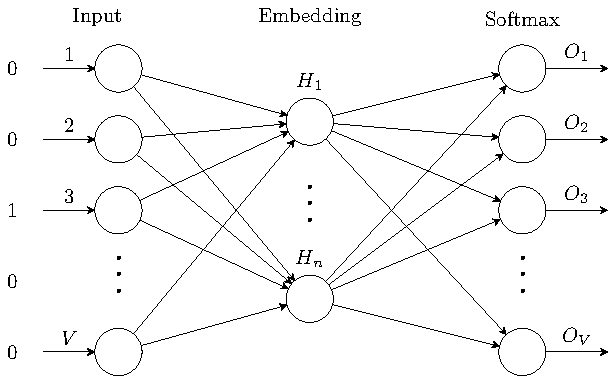
\includegraphics[scale=1,page=1]{Figures/wordembedding.pdf}
\caption{Neural network architecture for learnign COBW and skip-gram embeddings. A vocabulary is fed into the neural network using one-hot encoding methods. For a vocabulary of size V, the input vector is of size 1xV
 }
\end{figure}

The word representation/embedding can be calculated as 

$${w_i=x_iW}$$

${x_i}$ is the ${i^{th}}$ word in the dictionary, ${w_i}$ is the ${i^{th}}$ row in the input matrix ${W}$



\subsection{Word Representation using Neural Network}

\section{Cosine Similarity}

By looking at the Term-term matrix in Table. 1, we can see that data and scientist seems to have a common context word \textit{big} and could be close in their meanings. How can we quantify this? One possibility is using the dot-product of their vector representation.
$$
\vec{v}\cdot\vec{w}=\sum_{i=1}^N v_i w_i
$$

However, the dot-product favors vectors of higher frequency. Words that appears often are likely to have higher dot-product value than word of low occurence. To normalize the frequency, we can use cosine similarity meature, which is defined as below 
$$
cosine(\vec{v}, \vec{w})=\frac{\vec{v}\cdot\vec{w}}{|\vec{v}||\vec{w}|}=\frac{\sum_{i=1}^N v_i w_i}{\sqrt{\sum_1^N v_i^2}\sqrt{\sum_1^N w_i^2}}
$$




\section{Language Model}

\subsection{N-gram Language Models}
\begin{itemize}
\item Models that assign probabilities to sequences of words are called language models or LM.
\item An n-gram is a sequence of N words e.g. 2-gram (or bigram) "Good Morning", 3-gram "Turn it on"
\item N-gram lanuage models estimate the probability of the last word of an n-gram given the previous words
\end{itemize}

LM: What is the probability of having a sentence that consists a sequence of words: $w_1$, $w_2$, $w_3$ ... $w_N$, i.e. $P(w_1, w_2, w_3...w_N)$. 

Recall the chain rule:
\begin{align*}
&P(w_1, w_2, w_3...w_N)\\
&=P(w_1)P(w_2|w_1)P(w_3|w_1, w_2)P(w_4|w_1, w_2, w_3)...P(w_N|w_1, w_2, ...w_{N-1})
\end{align*}
In the case of bigram, we assume $P(w_N|w_1,...,w_{N-1})=P(w_N|w_{N-1})$, since the word is only dependent on the previous word, it is also called Markov assumption.
\vspace{0.2cm}
In general case of an n-gram, we assume $P(w_N|w_1, w_2, ...w_{N-1})=P(w_N|w_{N-1}, w_{N-2}, ...w_{N-n+1})$

\subsection{MLE Estimation for bigram }
In the case of bigram, the MLE estimation can be formulated as 
$$
P(w_N|w_{N-1})=\frac{C(w_{N-1}w_N)}{\sum_{w}C(w_{N-1}w)}=\frac{C(w_{N-1}w_N)}{C(w_{N-1})}
$$
Here, $C(w_{N-1})$ is the count of a word's occurence in a document. $C(w_{N-1}w_N)$ is the number of co-occurence of the word pair $w_{N-1}~w_{N}$, where $w_{N}$ appears after $w_{N-1}$ . For example, if we are interested in knowing the probabily that "$house$" occurs after "$white$", $P(house|white)$ we can do the followings: count the total occurence of the word "$white$" in a document and then count the co-occurence of the word pair "$white$ $house$"
 
\subsection{Example: MLE Estimation for bigram }
Estimate the bigram for the following corpus, here $\langle s \rangle$ and $\langle /s\rangle$ are introduced as the symbols that represents the begining and  end of a setence.

$\langle s \rangle$ \textit{I am Sam} $\langle /s\rangle$\\
$\langle s \rangle$ \textit{Sam I am} $\langle /s\rangle$\\
$\langle s \rangle$ \textit{I do not like green eggs and ham} $\langle /s \rangle$

We begin buy counting the words occurence and have $C(I)=3$, $C(Sam)=2$, $C(\langle /s\rangle)=3$, $C(\langle s\rangle)=3$, $C(\langle s \rangle I)=2$, $C(\langle s \rangle Sam)=1$

\vspace{0.2cm}

So we have $P(I|\langle s \rangle)=\frac{2}{3}$, $P(Sam|\langle s \rangle)=\frac{1}{3}$, $P(do|I)=\frac{1}{3}$, $P(am|I)=\frac{2}{3}$, $P(Sam|am)=\frac{1}{2}$, $P(\langle /s\rangle | Sam)=\frac{1}{2}$

\vspace{0.2cm}

The in-sample probability of $P(\langle s \rangle \textit{I am Sam}\langle /s\rangle)=P(I|\langle s \rangle)P(am|I)P(Sam|am)P(\langle /s\rangle | Sam)=\frac{2}{3} \times \frac{2}{3} \times \frac{1}{2} \times \frac{1}{2}=\frac{1}{9}$

\subsection{Compare LMs}
How do we compare two LM?
\begin{itemize}
\item A test data/hold out data set can be used to evaluate a LM. Apply the estiamated conditional probability to the test data set and compare the resulting probability.
\item More often than not, perplexity is used as a preferred metric, instead of the raw probability. Perplexity is defined as 
\begin{align*}
	PP(W)&=P(w_1, w_2, ...w_N)^{-\frac{1}{N}}\\
	&=\sqrt[N]{\frac{1}{P(w_1, w_2, ...w_N)}}
\end{align*}
\item Maximize probability is equivalent to minimize perplexity

\end{itemize}

\end{document}

